% Shared by main.tex (ACM layout) and arxiv.tex (arXiv layout).
\usepackage{array}
% Generated by scripts/paper_numbers.py from docs/findings. Do not edit.
% Percentages carry no % sign. Values with \times need math mode.
\newcommand{\AOrnithNatLongAmb}{11}
\newcommand{\AOrnithNatLongAmbHi}{20.8}
\newcommand{\AOrnithNatLongAmbLo}{6.3}
\newcommand{\AOrnithNatLongAmbN}{90}
\newcommand{\AOrnithNatLongAmbPct}{12.2}
\newcommand{\AOrnithNatLongExp}{0}
\newcommand{\AOrnithNatLongExpHi}{4.0}
\newcommand{\AOrnithNatLongExpLo}{0.0}
\newcommand{\AOrnithNatLongExpN}{90}
\newcommand{\AOrnithNatLongExpPct}{0.0}
\newcommand{\AOrnithNatShortAmb}{3}
\newcommand{\AOrnithNatShortAmbHi}{9.4}
\newcommand{\AOrnithNatShortAmbLo}{0.7}
\newcommand{\AOrnithNatShortAmbN}{90}
\newcommand{\AOrnithNatShortAmbPct}{3.3}
\newcommand{\AOrnithNatShortExp}{0}
\newcommand{\AOrnithNatShortExpHi}{4.0}
\newcommand{\AOrnithNatShortExpLo}{0.0}
\newcommand{\AOrnithNatShortExpN}{90}
\newcommand{\AOrnithNatShortExpPct}{0.0}
\newcommand{\AOrnithSnapLongAmb}{0}
\newcommand{\AOrnithSnapLongAmbHi}{4.0}
\newcommand{\AOrnithSnapLongAmbLo}{0.0}
\newcommand{\AOrnithSnapLongAmbN}{90}
\newcommand{\AOrnithSnapLongAmbPct}{0.0}
\newcommand{\AOrnithSnapLongExp}{0}
\newcommand{\AOrnithSnapLongExpHi}{4.0}
\newcommand{\AOrnithSnapLongExpLo}{0.0}
\newcommand{\AOrnithSnapLongExpN}{90}
\newcommand{\AOrnithSnapLongExpPct}{0.0}
\newcommand{\AOrnithSnapShortAmb}{0}
\newcommand{\AOrnithSnapShortAmbHi}{4.0}
\newcommand{\AOrnithSnapShortAmbLo}{0.0}
\newcommand{\AOrnithSnapShortAmbN}{90}
\newcommand{\AOrnithSnapShortAmbPct}{0.0}
\newcommand{\AOrnithSnapShortExp}{0}
\newcommand{\AOrnithSnapShortExpHi}{4.0}
\newcommand{\AOrnithSnapShortExpLo}{0.0}
\newcommand{\AOrnithSnapShortExpN}{90}
\newcommand{\AOrnithSnapShortExpPct}{0.0}
\newcommand{\AQwenNatLongAmb}{3}
\newcommand{\AQwenNatLongAmbHi}{9.4}
\newcommand{\AQwenNatLongAmbLo}{0.7}
\newcommand{\AQwenNatLongAmbN}{90}
\newcommand{\AQwenNatLongAmbPct}{3.3}
\newcommand{\AQwenNatLongExp}{0}
\newcommand{\AQwenNatLongExpHi}{4.0}
\newcommand{\AQwenNatLongExpLo}{0.0}
\newcommand{\AQwenNatLongExpN}{90}
\newcommand{\AQwenNatLongExpPct}{0.0}
\newcommand{\AQwenNatShortAmb}{4}
\newcommand{\AQwenNatShortAmbHi}{11.0}
\newcommand{\AQwenNatShortAmbLo}{1.2}
\newcommand{\AQwenNatShortAmbN}{90}
\newcommand{\AQwenNatShortAmbPct}{4.4}
\newcommand{\AQwenNatShortExp}{0}
\newcommand{\AQwenNatShortExpHi}{4.0}
\newcommand{\AQwenNatShortExpLo}{0.0}
\newcommand{\AQwenNatShortExpN}{90}
\newcommand{\AQwenNatShortExpPct}{0.0}
\newcommand{\AQwenSnapLongAmb}{0}
\newcommand{\AQwenSnapLongAmbHi}{4.0}
\newcommand{\AQwenSnapLongAmbLo}{0.0}
\newcommand{\AQwenSnapLongAmbN}{90}
\newcommand{\AQwenSnapLongAmbPct}{0.0}
\newcommand{\AQwenSnapLongExp}{0}
\newcommand{\AQwenSnapLongExpHi}{4.0}
\newcommand{\AQwenSnapLongExpLo}{0.0}
\newcommand{\AQwenSnapLongExpN}{90}
\newcommand{\AQwenSnapLongExpPct}{0.0}
\newcommand{\AQwenSnapShortAmb}{0}
\newcommand{\AQwenSnapShortAmbHi}{4.0}
\newcommand{\AQwenSnapShortAmbLo}{0.0}
\newcommand{\AQwenSnapShortAmbN}{90}
\newcommand{\AQwenSnapShortAmbPct}{0.0}
\newcommand{\AQwenSnapShortExp}{0}
\newcommand{\AQwenSnapShortExpHi}{4.0}
\newcommand{\AQwenSnapShortExpLo}{0.0}
\newcommand{\AQwenSnapShortExpN}{90}
\newcommand{\AQwenSnapShortExpPct}{0.0}
\newcommand{\ASparkNatLongAmb}{4}
\newcommand{\ASparkNatLongAmbHi}{11.0}
\newcommand{\ASparkNatLongAmbLo}{1.2}
\newcommand{\ASparkNatLongAmbN}{90}
\newcommand{\ASparkNatLongAmbPct}{4.4}
\newcommand{\ASparkNatLongExp}{0}
\newcommand{\ASparkNatLongExpHi}{4.0}
\newcommand{\ASparkNatLongExpLo}{0.0}
\newcommand{\ASparkNatLongExpN}{90}
\newcommand{\ASparkNatLongExpPct}{0.0}
\newcommand{\ASparkNatShortAmb}{2}
\newcommand{\ASparkNatShortAmbHi}{7.8}
\newcommand{\ASparkNatShortAmbLo}{0.3}
\newcommand{\ASparkNatShortAmbN}{90}
\newcommand{\ASparkNatShortAmbPct}{2.2}
\newcommand{\ASparkNatShortExp}{0}
\newcommand{\ASparkNatShortExpHi}{4.0}
\newcommand{\ASparkNatShortExpLo}{0.0}
\newcommand{\ASparkNatShortExpN}{90}
\newcommand{\ASparkNatShortExpPct}{0.0}
\newcommand{\ASparkSnapLongAmb}{3}
\newcommand{\ASparkSnapLongAmbHi}{9.4}
\newcommand{\ASparkSnapLongAmbLo}{0.7}
\newcommand{\ASparkSnapLongAmbN}{90}
\newcommand{\ASparkSnapLongAmbPct}{3.3}
\newcommand{\ASparkSnapLongExp}{0}
\newcommand{\ASparkSnapLongExpHi}{4.0}
\newcommand{\ASparkSnapLongExpLo}{0.0}
\newcommand{\ASparkSnapLongExpN}{90}
\newcommand{\ASparkSnapLongExpPct}{0.0}
\newcommand{\ASparkSnapShortAmb}{0}
\newcommand{\ASparkSnapShortAmbHi}{4.0}
\newcommand{\ASparkSnapShortAmbLo}{0.0}
\newcommand{\ASparkSnapShortAmbN}{90}
\newcommand{\ASparkSnapShortAmbPct}{0.0}
\newcommand{\ASparkSnapShortExp}{0}
\newcommand{\ASparkSnapShortExpHi}{4.0}
\newcommand{\ASparkSnapShortExpLo}{0.0}
\newcommand{\ASparkSnapShortExpN}{90}
\newcommand{\ASparkSnapShortExpPct}{0.0}
\newcommand{\CFiveEst}{6.3\times10^{-4}}
\newcommand{\CFiveHi}{4.3\times10^{-3}}
\newcommand{\CFiveLo}{-3.0\times10^{-3}}
\newcommand{\CFiveNeg}{96}
\newcommand{\CFivePos}{84}
\newcommand{\CFourEst}{3.0\times10^{-3}}
\newcommand{\CFourHi}{5.0\times10^{-3}}
\newcommand{\CFourLo}{1.3\times10^{-3}}
\newcommand{\CFourNeg}{56}
\newcommand{\CFourPos}{304}
\newcommand{\COneEst}{3.3\times10^{-3}}
\newcommand{\COneHi}{5.4\times10^{-3}}
\newcommand{\COneLo}{1.6\times10^{-3}}
\newcommand{\COneNeg}{0}
\newcommand{\COnePos}{360}
\newcommand{\CSixEst}{7.8\times10^{-2}}
\newcommand{\CSixHi}{1.2\times10^{-1}}
\newcommand{\CSixLo}{3.9\times10^{-2}}
\newcommand{\CSixNeg}{0}
\newcommand{\CSixPos}{14}
\newcommand{\CThreeEst}{1.1\times10^{-3}}
\newcommand{\CThreeHi}{3.6\times10^{-3}}
\newcommand{\CThreeLo}{-1.9\times10^{-3}}
\newcommand{\CThreeNeg}{69}
\newcommand{\CThreePos}{291}
\newcommand{\CTwoEst}{1.1\times10^{-3}}
\newcommand{\CTwoHi}{3.6\times10^{-3}}
\newcommand{\CTwoLo}{-1.9\times10^{-3}}
\newcommand{\CTwoNeg}{69}
\newcommand{\CTwoPos}{291}
\newcommand{\ChangesTotal}{30}
\newcommand{\ClaimedA}{7}
\newcommand{\DriftOrnithLongAmb}{1.5\times10^{-4}}
\newcommand{\DriftOrnithLongExp}{2.0\times10^{-6}}
\newcommand{\DriftOrnithShortAmb}{7.1\times10^{-5}}
\newcommand{\DriftOrnithShortExp}{2.4\times10^{-6}}
\newcommand{\DriftQwenLongAmb}{8.0\times10^{-6}}
\newcommand{\DriftQwenLongExp}{8.6\times10^{-8}}
\newcommand{\DriftQwenShortAmb}{1.4\times10^{-5}}
\newcommand{\DriftQwenShortExp}{9.0\times10^{-8}}
\newcommand{\DriftSparkLongAmb}{6.3\times10^{-5}}
\newcommand{\DriftSparkLongExp}{3.3\times10^{-8}}
\newcommand{\DriftSparkShortAmb}{6.6\times10^{-5}}
\newcommand{\DriftSparkShortExp}{3.0\times10^{-8}}
\newcommand{\ExplicitChanges}{0}
\newcommand{\ExplicitRestores}{1{,}080}
\newcommand{\ExplicitTurns}{540}
\newcommand{\FloorInexact}{0}
\newcommand{\GOneContradictions}{0}
\newcommand{\GOneRatio}{26}
\newcommand{\GOneRestores}{66}
\newcommand{\MarginAllConfident}{1}
\newcommand{\MarginAllConfidentN}{864}
\newcommand{\MarginAllConfidentPct}{0.1}
\newcommand{\MarginAllContested}{5}
\newcommand{\MarginAllContestedN}{143}
\newcommand{\MarginAllContestedPct}{3.5}
\newcommand{\MarginAllNearTie}{21}
\newcommand{\MarginAllNearTieN}{73}
\newcommand{\MarginAllNearTiePct}{29}
\newcommand{\MarginOrnithConfident}{0}
\newcommand{\MarginOrnithConfidentN}{269}
\newcommand{\MarginOrnithConfidentPct}{0}
\newcommand{\MarginOrnithContested}{2}
\newcommand{\MarginOrnithContestedN}{59}
\newcommand{\MarginOrnithContestedPct}{3}
\newcommand{\MarginOrnithNearTie}{12}
\newcommand{\MarginOrnithNearTieN}{32}
\newcommand{\MarginOrnithNearTiePct}{38}
\newcommand{\MarginQwenConfident}{1}
\newcommand{\MarginQwenConfidentN}{317}
\newcommand{\MarginQwenConfidentPct}{0}
\newcommand{\MarginQwenContested}{2}
\newcommand{\MarginQwenContestedN}{30}
\newcommand{\MarginQwenContestedPct}{7}
\newcommand{\MarginQwenNearTie}{4}
\newcommand{\MarginQwenNearTieN}{13}
\newcommand{\MarginQwenNearTiePct}{31}
\newcommand{\MarginSparkConfident}{0}
\newcommand{\MarginSparkConfidentN}{278}
\newcommand{\MarginSparkConfidentPct}{0}
\newcommand{\MarginSparkContested}{1}
\newcommand{\MarginSparkContestedN}{54}
\newcommand{\MarginSparkContestedPct}{2}
\newcommand{\MarginSparkNearTie}{5}
\newcommand{\MarginSparkNearTieN}{28}
\newcommand{\MarginSparkNearTiePct}{18}
\newcommand{\MembersA}{24}
\newcommand{\NatInexact}{1{,}080}
\newcommand{\NatTurns}{1{,}080}
\newcommand{\SnapCostMax}{443}
\newcommand{\SnapCostMin}{158}
\newcommand{\SnapCostOrnithLong}{272}
\newcommand{\SnapCostOrnithShort}{195}
\newcommand{\SnapCostQwenLong}{158}
\newcommand{\SnapCostQwenShort}{443}
\newcommand{\SnapCostSparkLong}{181}
\newcommand{\SnapCostSparkShort}{255}
\newcommand{\SnapInexactOrnith}{0}
\newcommand{\SnapInexactQwen}{0}
\newcommand{\SnapInexactSpark}{180}
\newcommand{\SnapValidOrnith}{360}
\newcommand{\SnapValidQwen}{360}
\newcommand{\SnapValidSpark}{360}
\newcommand{\SparkCases}{39}
\newcommand{\SparkContradictions}{0}
\newcommand{\TurnsPerModel}{360}
\newcommand{\TurnsTotal}{1{,}080}

\newcommand{\nub}{\texttt{n\_ubatch}}
\emergencystretch=2em
% End of the body: a label for the page check, and the number of body floats so far.
\providecommand\bodyfloats[2]{}
\makeatletter
\newcommand\markendofbody{\phantomsection\label{endofbody}%
  \immediate\write\@auxout{\string\bodyfloats{\arabic{figure}}{\arabic{table}}}}
\makeatother
\settopmatter{printacmref=false}
\setcopyright{none}
\renewcommand\footnotetextcopyrightpermission[1]{}
\begin{document}

\title[Cache Fidelity in llama.cpp]{Does Restoring a Prompt Cache Change What an Agent Does? A Pre-Registered Study of Cache Fidelity in llama.cpp}

\author{Manuel Gamal}
\affiliation{%
  \institution{Ain Shams University}
  \city{Cairo}
  \country{Egypt}}
\email{manuelaziz27@gmail.com}

\begin{abstract}
LLM agents resend a growing prompt on every turn, so serving stacks reuse
cached model state for nearly every request and assume the reuse does not
change the output. We test that assumption in a pre-registered study on
llama.cpp, comparing restored state with recomputation on \TurnsPerModel{}
synthetic agent turns with tool calls, for a hybrid recurrent, a sliding-window
and a dense model. Restoring at a natural turn boundary was never bit-exact
(\NatInexact{} of \NatTurns{} turns). It changed the agent's action on
\ASparkNatShortAmbPct--\AOrnithNatLongAmbPct\% of ambiguous requests on all
three models and on none of \ExplicitRestores{} explicit-request restores;
changes concentrated where the model's top two choices were nearly tied. An
exploratory experiment points to micro-batch tiling as the cause. Aligning the
reuse boundary to the micro-batch size made restores bit-exact on the hybrid
and dense models, at a median cost of \SnapCostMin--\SnapCostMax{}
re-evaluated tokens, but not on the sliding-window model at 4{,}096-token
boundaries. Results are for synthetic traffic, one engine build, one 4-bit
quantisation, one GPU and greedy decoding.
\end{abstract}


\ccsdesc[500]{Computing methodologies~Natural language processing}
\ccsdesc[300]{Computer systems organization~Reliability}
\keywords{LLM inference, prompt caching, KV cache, LLM agents, numerical reproducibility, llama.cpp}

\maketitle
\pagestyle{plain}

\section{Introduction}
\label{sec:intro}

Skeleton build: \NatInexact{} of \NatTurns{} natural-boundary restores were inexact,
and \AOrnithNatLongAmb{} of \AOrnithNatLongAmbN{} (\AOrnithNatLongAmbPct\%) changed the action.

\section{Background}
\label{sec:background}

\paragraph{Prefix reuse.}
A server that has processed a prompt keeps the resulting model state. When the
next prompt starts with the same tokens, it evaluates only the new suffix. In
llama.cpp this happens implicitly within a slot (\texttt{cache\_prompt}), and
explicitly through endpoints that save a slot's state to a file and restore
it~\cite{llamacpp-server}. We use explicit save and restore, because it lets us
force each condition and then prove from the server's own counters which one
ran. We call the number of reused tokens the \emph{reuse boundary} $k$.

\paragraph{Micro-batches.}
llama.cpp evaluates a prompt in physical micro-batches of \nub{} tokens
(512 in this study). A prompt of length $n$ is split into
$[0,U), [U,2U), \dots$ with $U = \nub$.

\paragraph{What the state is.}
The three models differ in what a cached prefix consists of.
Qwen3-4B~\cite{qwen3} is a dense transformer: the state is the keys and values
of every prefix position in every layer.
Spark-X2.5-4B~\cite{spark} interleaves three sliding-window attention layers
with one full-attention layer; according to the model file's metadata the
window is 512 tokens, so the windowed layers need only the most recent 512
positions.
Ornith-1.5-9B~\cite{ornith} is a hybrid: its model file declares the
\texttt{qwen35} architecture, with full attention in every fourth layer and
linear-attention layers in between that carry a fixed-size recurrent state.
The model card does not describe this structure and calls the model dense; we
rely on the file metadata (\texttt{full\_attention\_interval} of 4 and a
recurrent-state block). A
recurrent state summarises the whole prefix, so an error in it is carried
forward to every later token, where a per-position cache keeps errors local to
the positions that produced them.

\section{Method}
\label{sec:method}

\paragraph{Pre-registration.}
Seven hypotheses (H1--H7, Table~\ref{tab:hypotheses}), the outcomes, three
families of tests, the decision rules and a commitment to report a null result
were frozen in a tagged commit before any main-study turn ran~\cite{prereg}. The
analysis code was committed and tested on synthetic data before the run. At the
freeze we had seen restore only on raw-text prompts in two gate experiments
(G0, G1), and chat-templated agent traffic only on the recompute path (G2).

\paragraph{Evidence labels.}
\label{sec:labels}
We label every result. \emph{Confirmatory} results are the pre-registered test
families A, B and C and the hypotheses. \emph{Pre-registered secondary} results
are analyses the plan listed with intervals only and no corrected test.
\emph{Exploratory} results were not pre-registered: the gates that ran before
the freeze, and a follow-up that ran after the main study.

\begin{table}[t]
\caption{Models and prompt sizes. All models are Q4\_K\_M quantisations. Token
counts are medians over 180 turns per band; the snapped boundary is the natural
boundary rounded down to a multiple of 512.}
\label{tab:setup}
% src: docs/findings/2026-09-10-study-manifest.md, "Measured"
\small
\begin{tabular}{@{}llrrrr@{}}
\toprule
 & & \multicolumn{2}{c}{Prompt tokens} & \multicolumn{2}{c}{Snapped $k$} \\
Model & Cached state & short & long & short & long \\
\midrule
Ornith-1.5-9B & hybrid recurrent & 1{,}245 & 6{,}439 & 1{,}024 & 6{,}144 \\
Spark-X2.5-4B & sliding window & 786 & 4{,}298 & 512 & 4{,}096 \\
Qwen3-4B & dense & 992 & 5{,}316 & 512 & 5{,}120 \\
\bottomrule
\end{tabular}
\end{table}

\paragraph{Models and engine.}
Table~\ref{tab:setup} lists the models. All runs use \texttt{llama-server},
build \texttt{b10839}, on one RTX 4060 Laptop GPU (8\,GB) with all layers
offloaded, a context of 8{,}192 tokens, one slot, $\nub = 512$, and the
server's own prompt cache and context checkpoints disabled. Spark additionally
runs with \texttt{-{}-swa-full}. Decoding is greedy, for at most 192 new tokens,
recording the top-10 log-probabilities at every generated position.

\paragraph{Traffic.}
We generate 90 base conversations between a user and an agent with three
deterministic mock tools (look up a record, sum a list of numbers, format a
report). Each conversation is a sequence of completed tool round trips, rendered
through the model's own chat template with the tool schemas. Each base appears
with a short history (8 round trips) and a long one (60), and ends with either
an \emph{explicit} request (``Look up record 153'') or an \emph{ambiguous} one
drawn from five types (for example ``Add up the numbers from earlier''). That
gives \TurnsPerModel{} turns per model, and every model receives the same turns.

\paragraph{Boundaries and arms.}
The \emph{natural} boundary of a turn is the longest common token prefix of the
history rendered alone and the full prompt, which is what a server can reuse.
(Qwen3's template renders the last assistant message differently once a new user
message follows, so the history is not itself a prefix.) The \emph{snapped}
boundary is $k - (k \bmod 512)$. Each turn runs six arms: recompute, restore at
the natural boundary and restore at the snapped boundary, each twice. A restore
arm evaluates the first $k$ tokens, saves the slot, erases it, restores it and
then completes the prompt.

\paragraph{Arm proofs.}
A server can silently reprocess a prompt it was asked to restore. A restore arm
therefore counts only if the server reports evaluating exactly the suffix and
the saved slot holds exactly $k$ tokens; a recompute arm counts only if the
server reports evaluating the whole prompt.
% src: docs/findings/2026-09-11-main-study.md, "Validity"
All 6{,}480 arms passed. Further safeguards are in Appendix~\ref{app:safeguards}.

\paragraph{Outcomes.}
The primary outcome is an \emph{action change}: the restore arm's action differs
from the recompute arm's in both replicates. An action is the first complete
tool call, with its name and canonical arguments, or no call. Secondary outcomes
are bit-exactness (identical tokens and bitwise-identical top-10
log-probabilities at every position) and distribution drift, the per-turn mean
and maximum Jensen--Shannon divergence (JSD) over positions where both arms
share the same context. The \emph{action margin} is a covariate: the smallest
gap between the top two log-probabilities over the positions that decide the
action, on the recompute arm, binned as near-tie ($<0.5$ nats), contested
(0.5--2) and confident ($\geq 2$).

\paragraph{Tests.}
The noise floor is measured: recompute runs twice per turn. When the floor is
zero, a single reproducible change cannot arise under the null, so the test
rejects and the Clopper--Pearson interval~\cite{clopper-pearson} carries the
size. Family~A (24 members) tests action changes per model, boundary, history
length and request type; family~B (16) tests drift on the hybrid; family~C (6)
tests paired contrasts with exact sign tests and bootstrap intervals. The Holm
correction~\cite{holm} is applied within each family. An effect is claimed only
if the test rejects and its interval excludes zero.

\section{Results}
\label{sec:results}

\paragraph{Validity.}
All \TurnsPerModel{} turns completed on each model and no turn was excluded.
The two recompute arms were bit-identical on every turn (\FloorInexact{} of
\TurnsTotal{} differed), so the engine was deterministic and any difference is
attributable to restore. Every restore result reproduced in its second
replicate, and no action change appeared in only one replicate.

\paragraph{Exactness.}
At natural boundaries, \NatInexact{} of \NatTurns{} restores were not
bit-exact (a descriptive count). That includes all \ExplicitTurns{} explicit-request turns, where
restore and recompute generated identical tokens but never identical
log-probabilities. At snapped boundaries (confirmatory, H1) every restore was bit-exact on Ornith
and on Qwen3 (\SnapValidOrnith{} of \SnapValidOrnith{} turns each). On Spark,
the 180 short-history turns were exact and all \SnapInexactSpark{} long-history
turns were not, which falsifies H1 for that model.

\begin{figure}[t]
\centering
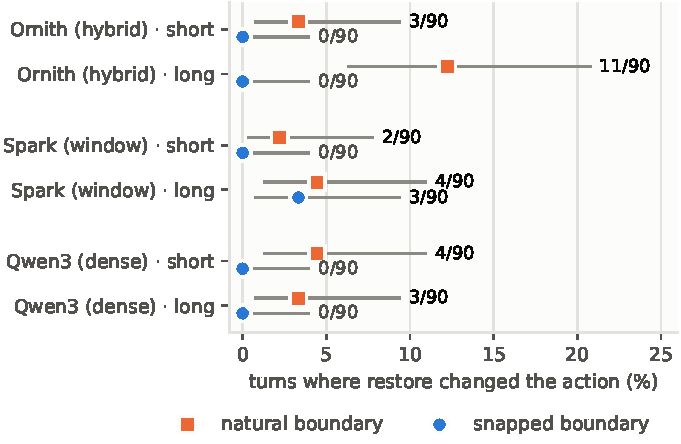
\includegraphics[width=\columnwidth]{figures/action_changes.pdf}
\caption{Turns on which restore changed the agent's action, on ambiguous
requests (confirmatory, family~A). Each point is 90 turns; bars are 95\%
Clopper--Pearson intervals. Ornith is the hybrid recurrent model, Spark the
sliding-window model, Qwen3 the dense model. On explicit requests there were
\ExplicitChanges{} changes in \ExplicitRestores{} restores.}
\label{fig:actions}
\end{figure}

\paragraph{Action changes (confirmatory).}
Figure~\ref{fig:actions} shows family~A. At natural boundaries, restore changed
the action on ambiguous requests on every model:
on Ornith, \AOrnithNatShortAmb{} of \AOrnithNatShortAmbN{} short-history turns
(\AOrnithNatShortAmbPct\%, 95\% CI \AOrnithNatShortAmbLo--\AOrnithNatShortAmbHi\%)
and \AOrnithNatLongAmb{} of \AOrnithNatLongAmbN{} long-history turns
(\AOrnithNatLongAmbPct\%, CI \AOrnithNatLongAmbLo--\AOrnithNatLongAmbHi\%);
on Spark, \ASparkNatShortAmb{} (\ASparkNatShortAmbPct\%) and
\ASparkNatLongAmb{} (\ASparkNatLongAmbPct\%);
on Qwen3, \AQwenNatShortAmb{} (\AQwenNatShortAmbPct\%) and
\AQwenNatLongAmb{} (\AQwenNatLongAmbPct\%).
No explicit request changed: \ExplicitChanges{} of \ExplicitRestores{} restores,
with a 95\% upper bound of \AOrnithNatShortExpHi\% per cell of 90. At snapped
boundaries the only changes were \ASparkSnapLongAmb{} on Spark's long
histories. In total \ClaimedA{} of the \MembersA{} family members are claimed.
The dense and sliding-window models changed actions too, at rates similar to
the hybrid's on short histories. The study pre-registered no test that compares
action-change rates between architectures, and with 2--11 events per cell the
intervals overlap widely.

\begin{figure}[t]
\centering
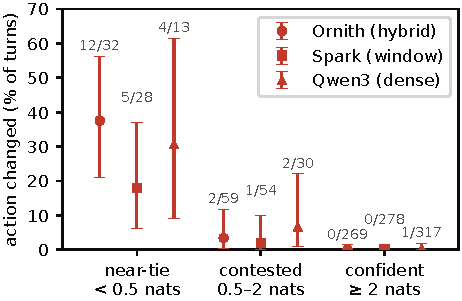
\includegraphics[width=\columnwidth]{figures/margin_bins.pdf}
\caption{Action changes at natural boundaries by the recompute arm's action
margin (pre-registered secondary; intervals only). Labels give changed turns
over turns in the bin; bars are 95\% Clopper--Pearson intervals.}
\label{fig:margins}
\end{figure}

\paragraph{Where the changes happen (pre-registered secondary).}
Figure~\ref{fig:margins} groups natural-boundary turns by action margin. Pooled
over models, restore changed the action on \MarginAllNearTie{} of
\MarginAllNearTieN{} near-tie turns (\MarginAllNearTiePct\%), \MarginAllContested{}
of \MarginAllContestedN{} contested turns (\MarginAllContestedPct\%) and
\MarginAllConfident{} of \MarginAllConfidentN{} confident turns
(\MarginAllConfidentPct\%). The predicted ordering holds on each model. This
analysis was pre-registered with intervals only, so it is descriptive.

\paragraph{What changed (descriptive).}
% src: docs/findings/2026-09-11-main-study.md, "Where the changes happen"; recounted from docs/findings/study/changed_turns.json
Of the \ChangesTotal{} changes, 11 were the same tool called with different
arguments, 10 were a tool call that became a text reply, and 9 were a text
reply or clarifying question that became a tool call. None switched to a
different tool. In one case both arms summed a list of 23 numbers from the
history, but the restore arm omitted one of them, so the tool returned a
different total (Appendix~\ref{app:examples}).

\paragraph{Distribution drift (confirmatory).}
Restore shifted the hybrid's output distribution at every natural boundary
(family~B, all eight natural-boundary members claimed; H2). On explicit
requests with short histories the median per-turn mean JSD (descriptive) was
$\DriftOrnithShortExp$ on Ornith against $\DriftQwenShortExp$ on Qwen3 and
$\DriftSparkShortExp$ on Spark. Of the six contrasts in family~C, three are
claimed: snapping removes drift on the hybrid (C1), the hybrid drifts more than
the sliding-window model (C4), and action changes are more frequent on
ambiguous than explicit requests (C6). The hybrid drifted more than the dense
model on \CThreePos{} of 360 turns, but the interval of the mean difference
includes zero ($[\CThreeLo, \CThreeHi]$), so C3 is not claimed: a few
dense-model turns drifted heavily. Drift was not shown
to grow with history length (C5). The models see different prompt lengths for
the same conversation (Table~\ref{tab:setup}); in an exploratory check within
each history length, the hybrid still drifted more than the sliding-window
model.
Appendix~\ref{app:families} has the full tables.

\begin{table}[t]
\caption{Pre-registered hypotheses and verdicts. A hypothesis is supported only
if every test it names is claimed.}
\label{tab:hypotheses}
% src: docs/findings/2026-09-11-main-study.md, "Hypotheses"
\small
\begin{tabular}{@{}l>{\raggedright\arraybackslash}p{0.46\columnwidth}>{\raggedright\arraybackslash}p{0.36\columnwidth}@{}}
\toprule
 & Hypothesis & Verdict \\
\midrule
H1 & Snapped restores are bit-exact on every model & Holds on hybrid and dense; \textbf{fails} on sliding window \\
H2 & Restore shifts the hybrid's output distribution & Supported \\
H3 & Restore changes the hybrid's actions & Partial: ambiguous requests only \\
H4 & The hybrid diverges more than both controls & Partial: more than sliding window; not shown for dense \\
H5 & Snapping helps, more on the hybrid than the dense model & Partial: helps; a larger effect on the hybrid not shown \\
H6 & Divergence grows with history length & \textbf{Not supported} \\
H7 & Action changes concentrate in ambiguous requests & Supported \\
\bottomrule
\end{tabular}
\end{table}

\section{Mechanism and Mitigation}
\label{sec:mechanism}

\begin{figure*}[t]
\centering
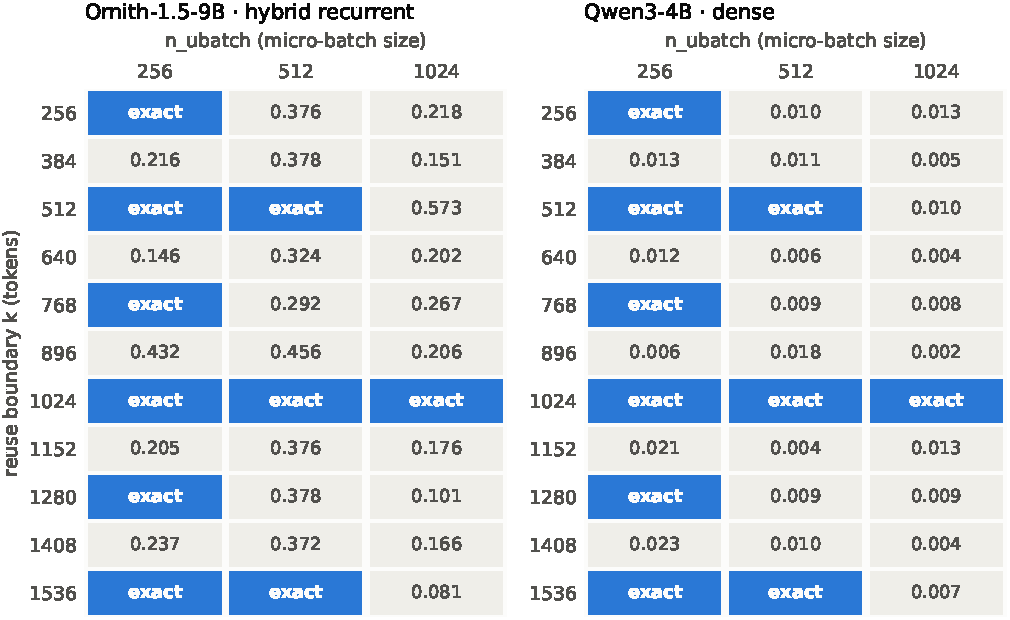
\includegraphics[width=0.82\textwidth]{figures/g1_exactness_grid.pdf}
% src: docs/findings/2026-09-10-g1.md, "Setup" (1,911 and 1,793 prompt tokens; 11 boundaries; 16 new tokens)
\caption{Restore is bit-exact when the reuse boundary $k$ is a multiple of
\nub{} (exploratory, gate G1). One prompt of 1.8--1.9K tokens per model,
11 boundaries, three micro-batch sizes. Inexact cells show the largest total
variation distance from recompute over 16 generated positions.}
\label{fig:grid}
\end{figure*}

\paragraph{Micro-batch tiling.}
Restoring a saved slot returns the bytes that were saved, so the restore itself
adds no error. The difference comes from how the prompt is split into
micro-batches. Recompute tiles the whole prompt from position 0:
$[0,U), [U,2U), \dots$ Restore tiled the prefix $[0,k)$ when it was cached, and
then tiles the suffix afresh starting at $k$. The two tilings coincide only when
$k$ is a multiple of $U$. Otherwise the same matrix products, attention sums and
recurrent updates are accumulated in a different order, and floating-point
addition is not associative~\cite{tml-nondeterminism,yuan-nondeterminism}.

\paragraph{Test (exploratory).}
The gate experiment G1, run before the pre-registration, tested this prediction
by changing \nub. If tiling is the cause, the set of exact boundaries must move
with it: $k = 512$ is exact at $\nub = 256$ and 512 but not at 1{,}024;
$k = 768$ only at 256. Figure~\ref{fig:grid} shows the outcome on the hybrid
and the dense model: all \GOneRestores{} restores matched the prediction, with
\GOneContradictions{} exceptions. The inexact cells are about \GOneRatio{}
times larger on the hybrid by median, consistent with a recurrent state
carrying the error forward. This evidence rests on one raw-text prompt per
model.

\paragraph{Mitigation: snapping (confirmatory).}
The rule suggests a fix that needs no change to the engine: round the reuse
boundary down to a multiple of \nub{} and re-evaluate the remainder. In the
main study this made every restore bit-exact on Ornith and Qwen3, which removed
all drift and every action change on those models (H1; contrast C1). The cost
is the re-evaluated remainder: a median of \SnapCostOrnithShort{} and
\SnapCostOrnithLong{} tokens per turn on Ornith (short and long histories),
\SnapCostQwenShort{} and \SnapCostQwenLong{} on Qwen3, and at most 511 by
construction.

\paragraph{Where snapping fails.}
On Spark, snapped restores were exact at $k = 512$ and inexact at $k = 4{,}096$,
on all \SnapInexactSpark{} long-history turns, and \ASparkSnapLongAmb{} action
changes remained. Alignment to \nub{} is therefore not sufficient on the
sliding-window model. An exploratory follow-up on one 4{,}268-token prompt
varied \nub{} over 256, 512 and 1{,}024.
% src: docs/findings/2026-09-11-spark-window.md, "Exact grid", "The rules", "Diagnostics"
With the default configuration, a restore was exact only when the boundary was
aligned \emph{and} lay within the 512-token attention window:
\SparkContradictions{} exceptions in \SparkCases{} cases. Disabling flash
attention extended exactness to 2{,}560 tokens but not beyond. Without
\texttt{-{}-swa-full} the server discarded every restored state and recomputed
the prompt, so outputs matched recompute exactly; only the arm proofs revealed
that no restore had taken place. We have located this behaviour but not
explained it (Appendix~\ref{app:spark}).

\section{Limitations}
\label{sec:limits}

\paragraph{Expectations that failed.}
Four expectations did not hold. (1)~Our design document, written before the
data, expected action changes on the hybrid and none on the dense and
sliding-window controls; all three changed actions, at similar rates on short
histories. Restore-induced action changes appear to be a property of near-tie
decisions, not of recurrent state alone. (2)~We pre-registered that snapping
would be exact on every model (H1); on the sliding-window model it was inexact
at every 4{,}096-token boundary. (3)~Drift was not shown to grow with history
length on the hybrid (H6). (4)~The hybrid's mean drift was not shown to exceed
the dense model's (C3), although it was larger on most turns.

\paragraph{Scope.}
One engine build, one quantisation (Q4\_K\_M), one GPU, $\nub = 512$, three
models. Exactness is a property of numerical kernels and can differ on other
builds, backends and hardware. We make no claim about other inference engines.

\paragraph{Traffic.}
The traffic is synthetic: three mock tools and five ambiguous request types.
Real agent traffic may contain more or fewer near-tie decisions. The relation
between action margin and action change is the part we expect to transfer; the
rates are not.

\paragraph{Few events.}
Each rate rests on 2--11 changed turns out of 90, so the intervals are wide.
No test compares action-change rates between architectures, and the larger
count on the hybrid's long histories (11 against 3) is descriptive.

\paragraph{Decoding.}
Decoding was greedy. Under sampling, drift would shift sampled tokens instead
of flipping the most likely one; we did not measure that.

\paragraph{Exploratory evidence.}
The tiling mechanism (G1) and the sliding-window rule each rest on a single
prompt per configuration and were not pre-registered. The cause of the
sliding-window behaviour inside llama.cpp is not identified.

\section{Related Work}
\label{sec:related}

\paragraph{Cache nondeterminism in the engine.}
The llama.cpp server documentation states that prompt caching can make results
nondeterministic because logits differ across batch
sizes~\cite{llamacpp-server}. We do not claim to have discovered that. We
measure when reuse is exact, how the difference varies with architecture,
whether it changes agent actions, and what a mitigation costs.

\paragraph{Cached versus recomputed outputs.}
Chodavarapu and Xu find that KV-cached and cache-free decoding diverge on every
token under FP16 and that FP32 removes the token flips~\cite{chodavarapu-fp16};
Lorup finds the same for a retained cache against a re-prefill in BF16 and
shows that the boundary cache carries the divergent
trajectory~\cite{lorup-stage-replay}. Closest to our work, Patodiya runs a
multi-turn agentic tool-use workload on llama.cpp and vLLM and finds that
cache-hit and recompute paths diverge, increasingly with weight
quantisation~\cite{patodiya-cache-divergence}. That study measures divergence
of trajectories on dense models; we measure changes in the agent's action,
compare hybrid recurrent, sliding-window and dense state, identify the
micro-batch alignment that makes reuse exact, and test a mitigation. Zhang and
Yang reach a changed action by another route: a KV cache kept after an
aborted branch, with the decision tokens held identical, flipped a protected
tool effect in 25 of 63 audited cells, and rebuilding the cache removed
it~\cite{zhang-rollback}. There the cache holds content that the transcript no
longer contains; in our study the cached and recomputed paths see the same
tokens. Concurrently, Gu et al.\ show that approximate, non-prefix KV reuse
makes answers depend on the order of earlier requests~\cite{gu-request-order}.

\paragraph{Numerical nondeterminism.}
He et al.\ trace nondeterminism in LLM serving to kernels whose results depend
on batch size~\cite{tml-nondeterminism}, and Yuan et al.\ show that
floating-point non-associativity changes outputs across batch sizes and
hardware~\cite{yuan-nondeterminism}. vLLM ships a batch-invariant
mode~\cite{vllm-batch-invariant}, and SGLang aligns chunked-prefill
truncation points to a multiple of the split-KV size for
determinism~\cite{sglang-deterministic}. Micro-batch tiling at a reuse boundary is an
instance of the same effect, reached through the prompt cache.

\paragraph{Agent workloads and caching.}
TraceLab characterises coding-agent traces and their prefix-cache hit
rates~\cite{tracelab}; other work improves hit rates and latency for agent
traffic~\cite{vllm-mooncake,policy-runtime}. These studies measure speed. Ours
measures whether the reused state yields the same output.

\paragraph{Hybrid models and prefix caching.}
Prefix caching for hybrid models has been troublesome in several engines. A
llama.cpp issue, since closed, reported full prompt reprocessing on every turn
for a hybrid model~\cite{llamacpp-20225}. vLLM tracks hybrid prefix caching in
an open issue~\cite{vllm-26201}, with reports that caching works only in
blocks of 528 tokens~\cite{vllm-40696} and misses on incremental multimodal
requests~\cite{vllm-43587}. An SGLang roadmap describes its cache's
compatibility with hybrid models as limited~\cite{sglang-21846}. The LMCache
documentation notes that for hybrid models generation ``is not bit-exact
between a cached and a fresh run''~\cite{lmcache-hybrid}, without quantifying
the difference.

\section{Conclusion}
\label{sec:conclusion}

On one build of llama.cpp, restoring cached state at a natural agent-turn
boundary was never bit-exact, and it changed the agent's action on a few
percent of ambiguous requests on hybrid, sliding-window and dense models alike,
almost always where the model was already close to a tie. The cause we
identified is the tiling of the prompt into micro-batches. Aligning the reuse
boundary to the micro-batch size restores exactness on the hybrid and dense
models for a few hundred re-evaluated tokens per turn, but not on the
sliding-window model once the prefix exceeds its window. A serving stack can
apply the alignment today where the architecture allows it, and can treat
low-margin decisions as the ones exposed to cache reuse. The cause of the
sliding-window behaviour, and whether other engines behave the same way, remain
open.

% DRAFT WORDING: Manuel to confirm that this describes what actually happened.
\begin{acks}
The author used Claude (Anthropic), an AI assistant, to help write the measurement
code and to draft and edit this text. Numbers in the text are generated from
the recorded result files. The author designed the study, ran the experiments,
and is responsible for the content.
\end{acks}


\markendofbody

\bibliographystyle{ACM-Reference-Format}
\bibliography{refs}

\appendix
\section{Families B and C in Full}
\label{app:families}

Table~\ref{tab:drift} gives the median drift at natural boundaries. Family~B
tests the hybrid only; the other two models are shown for reference. At snapped
boundaries drift was exactly zero on Ornith and Qwen3 in every condition.
Table~\ref{tab:contrasts} gives the six contrasts of family~C. C2 and C3 are
numerically identical because snapped drift was exactly zero on both the hybrid
and the dense model, so the interaction reduces to the natural-boundary
difference.

\begin{table}[h]
\caption{Median per-turn mean JSD at natural boundaries, 90 turns per cell
(descriptive; the pre-registered family~B estimate is the mean).}
\label{tab:drift}
\small
\begin{tabular}{@{}lcccc@{}}
\toprule
 & \multicolumn{2}{c}{Short history} & \multicolumn{2}{c}{Long history} \\
Model & explicit & ambiguous & explicit & ambiguous \\
\midrule
Ornith & $\DriftOrnithShortExp$ & $\DriftOrnithShortAmb$ & $\DriftOrnithLongExp$ & $\DriftOrnithLongAmb$ \\
Spark & $\DriftSparkShortExp$ & $\DriftSparkShortAmb$ & $\DriftSparkLongExp$ & $\DriftSparkLongAmb$ \\
Qwen3 & $\DriftQwenShortExp$ & $\DriftQwenShortAmb$ & $\DriftQwenLongExp$ & $\DriftQwenLongAmb$ \\
\bottomrule
\end{tabular}
\end{table}

\begin{table*}[t]
\caption{Family~C: mechanism contrasts (confirmatory). ``More / less'' counts
the turns on which the first side of the contrast was larger or smaller. The
estimate is the mean paired difference in per-turn mean JSD, except for C6,
which is a difference in action-change rate in percentage points. Intervals are 95\% paired
bootstrap intervals.}
\label{tab:contrasts}
% src for the Pairs and Claimed columns: docs/findings/2026-09-11-main-study.md, "Family C"
\small
\begin{tabular}{@{}llrrrll@{}}
\toprule
 & Contrast & Pairs & More & Less & Estimate and 95\% interval & Claimed \\
\midrule
C1 & Snapping on the hybrid (natural $-$ snapped) & 360 & \COnePos & \COneNeg & $\COneEst$ \ $[\COneLo,\ \COneHi]$ & yes \\
C2 & Snapping $\times$ architecture (hybrid vs.\ dense) & 360 & \CTwoPos & \CTwoNeg & $\CTwoEst$ \ $[\CTwoLo,\ \CTwoHi]$ & no \\
C3 & Hybrid $-$ dense, natural boundary & 360 & \CThreePos & \CThreeNeg & $\CThreeEst$ \ $[\CThreeLo,\ \CThreeHi]$ & no \\
C4 & Hybrid $-$ sliding window, natural boundary & 360 & \CFourPos & \CFourNeg & $\CFourEst$ \ $[\CFourLo,\ \CFourHi]$ & yes \\
C5 & Long $-$ short history on the hybrid & 180 & \CFivePos & \CFiveNeg & $\CFiveEst$ \ $[\CFiveLo,\ \CFiveHi]$ & no \\
C6 & Ambiguous $-$ explicit on the hybrid (action change) & 180 & \CSixPos & \CSixNeg & \CSixEstPct{} \ [\CSixLoPct,\ \CSixHiPct] points & yes \\
\bottomrule
\end{tabular}
\end{table*}

\section{Per-Turn Drift}
\label{app:drift}

Figure~\ref{fig:drift} shows the drift of every natural-boundary turn.

\begin{figure}[h]
\centering
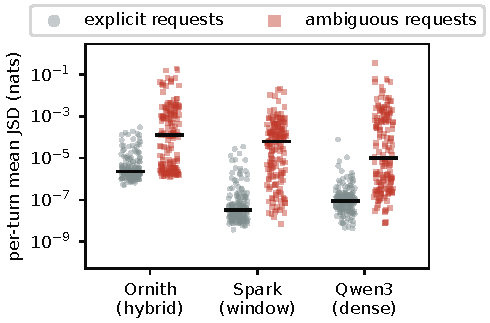
\includegraphics[width=\columnwidth]{figures/drift_per_turn.pdf}
\caption{Per-turn mean JSD between restore and recompute at natural
boundaries, one point per turn, both history lengths. Black bars are
medians pooled over both history lengths (descriptive). Ornith is the hybrid recurrent model, Spark the sliding-window model,
Qwen3 the dense model.}
\label{fig:drift}
\end{figure}

\section{Sliding-Window Follow-Up}
\label{app:spark}

This follow-up is exploratory. Its plan and predictions were committed before
it ran, but it was not part of the pre-registration, and it uses one prompt:
the first long-history main-study turn, 4{,}268 tokens, with 13 reuse
boundaries and 16 generated tokens per case. Table~\ref{tab:sparkgrid} shows
which restores were bit-exact. With default settings, the rule ``exact when
$k$ is a multiple of \nub{} and $k \leq 512$'' fits all \SparkCases{} cases.
The alternatives fit worse: ``aligned and $k \leq \nub$'' fails twice,
``$k \leq 512$ regardless of alignment'' six times, and alignment alone 20
times. In a fifth run without \texttt{-{}-swa-full}, the server saved each slot
correctly but then evaluated the whole prompt on all 13 restores, so no restore
was proven and every output equalled recompute.

\begin{table}[h]
\caption{Spark: bit-exact (E) or inexact (--) restores by reuse boundary $k$
and server configuration (exploratory). FA off: flash attention disabled.}
\label{tab:sparkgrid}
% src: docs/findings/2026-09-11-spark-window.md, "Exact grid"
\small
\begin{tabular}{@{}rcccc@{}}
\toprule
 & \multicolumn{3}{c}{\nub{} (default settings)} & FA off \\
$k$ & 256 & 512 & 1{,}024 & 512 \\
\midrule
256 & E & -- & -- & -- \\
384 & -- & -- & -- & -- \\
512 & E & E & -- & E \\
640 & -- & -- & -- & -- \\
768 & -- & -- & -- & -- \\
1{,}024 & -- & -- & -- & E \\
1{,}280 & -- & -- & -- & -- \\
1{,}536 & -- & -- & -- & E \\
2{,}048 & -- & -- & -- & E \\
2{,}560 & -- & -- & -- & E \\
3{,}072 & -- & -- & -- & -- \\
3{,}584 & -- & -- & -- & -- \\
4{,}096 & -- & -- & -- & -- \\
\bottomrule
\end{tabular}
\end{table}

\section{Changed Actions}
\label{app:examples}

% src: docs/findings/study/changed_turns.json; probabilities from data/study/*.jsonl (replicate 1, top-10 log-probabilities)
Table~\ref{tab:examples} shows three changed turns side by side, all on Ornith
at natural boundaries, and Table~\ref{tab:census} lists all \ChangesTotal{}.
Decoding is greedy, so each arm emits its more probable token, and every change
reproduced in both replicates. The two request types that ask the model to
choose between tools produced no changes.

\begin{table*}[p]
\caption{Three changed turns on Ornith at natural boundaries. ``At
token'' gives the two most probable tokens, with probabilities in
percent, at the first generated position where the arms differ; \textsc{call}
is the token that opens a tool call. Values in bold are where the outputs
part.}
\label{tab:examples}
\small
\begin{tabular}{@{}>{\raggedright\arraybackslash}p{0.15\textwidth}>{\raggedright\arraybackslash}p{0.39\textwidth}>{\raggedright\arraybackslash}p{0.39\textwidth}@{}}
\toprule
 & Recompute & Restore \\
\midrule
\multicolumn{3}{@{}l}{\textit{(a) Long history, ``Pull up that record again'', $k=6{,}416$, action margin 0.09}} \\
At token 0 & \textbf{\textsc{call} 41.0}, `The' 37.4 & \textbf{`The' 53.3}, \textsc{call} 40.3 \\
Output & calls \texttt{lookup\_record(73)} & ``The record you're referring to is record 73, which has field=beta value=701.'' \\
\midrule
\multicolumn{3}{@{}l}{\textit{(b) Short history, ``Write that up for me'', $k=1{,}212$, action margin 0.61}} \\
At token 0 & \textbf{`I' 44.6}, \textsc{call} 24.2 & \textbf{\textsc{call} 34.0}, another token 28.8 \\
Output & ``I'm not sure which task or information you're referring to. Could you clarify what you'd like me to write up?'' & calls \texttt{format\_report} with the title ``Record Lookup Summary'' and three records from the history \\
\midrule
\multicolumn{3}{@{}l}{\textit{(c) Long history, ``Add up the numbers from earlier'', $k=6{,}351$, action margin 0.22}} \\
At token 38 & \textbf{`6' 55.4}, `9' 44.4 & \textbf{`9' 65.4}, `6' 34.3 \\
Output & \texttt{compute\_sum([68, 110, 72, 118, 36, \textbf{65}, 90, \ldots, 74])}, 23 values & \texttt{compute\_sum([68, 110, 72, 118, 36, \textbf{90}, \ldots, 74])}, 22 values; 65 is missing \\
\bottomrule
\end{tabular}

\bigskip
\caption{All \ChangesTotal{} changed actions. History: prefix band. Request:
``Add up the numbers from earlier'', ``Pull up that record again'' or ``Write
that up for me''. $k$: reuse boundary. Pos.: first generated position where
the arms differ. The two token columns give the two most probable tokens there,
with probabilities in percent; \textsc{call} opens a tool call and
\textit{other} is a token that neither arm emitted. Arguments: the same tool
with different arguments. The three snapped rows are Spark at
$k=4{,}096$, where snapping is not exact (\S\ref{sec:mechanism}). Turn
identifiers and full outputs are in the repository.}
\label{tab:census}
\footnotesize
\setlength{\tabcolsep}{4pt}
\begin{tabular}{@{}llllrrrlll@{}}
\toprule
Model & History & Request & Boundary & $k$ & Margin & Pos. & Recompute top two & Restore top two & Change \\
\midrule
Ornith & long & Add up & natural & 6{,}387 & 0.07 & 29 & `7' 35.6, `2' 33.4 & `2' 46.9, `9' 31.5 & arguments \\
Ornith & long & Record & natural & 6{,}388 & 1.44 & 0 & \textsc{call} 76.9, \textit{other} 18.1 & `I' 37.9, \textit{other} 32.6 & tool$\to$text \\
Ornith & long & Add up & natural & 6{,}467 & 0.21 & 16 & `6' 53.6, `2' 42.4 & `2' 60.4, `6' 34.2 & tool$\to$text \\
Ornith & long & Record & natural & 6{,}294 & 0.13 & 0 & \textsc{call} 45.3, `The' 39.6 & `The' 63.1, \textsc{call} 22.8 & tool$\to$text \\
Ornith & long & Add up & natural & 6{,}420 & 0.03 & 55 & `9' 58.2, `3' 41.0 & `3' 53.0, `9' 46.3 & arguments \\
Ornith & long & Add up & natural & 6{,}482 & 0.03 & 30 & `5' 55.0, `6' 45.0 & `6' 50.8, `5' 49.2 & arguments \\
Ornith & long & Add up & natural & 6{,}506 & $<$0.01 & 16 & `6' 46.3, `2' 45.9 & `2' 65.9, `6' 24.5 & arguments \\
Ornith & long & Record & natural & 6{,}416 & 0.09 & 0 & \textsc{call} 41.0, `The' 37.4 & `The' 53.3, \textsc{call} 40.3 & tool$\to$text \\
Ornith & long & Add up & natural & 6{,}515 & 0.06 & 130 & `8' 46.2, `4' 43.4 & `4' 45.9, `8' 44.2 & arguments \\
Ornith & long & Add up & natural & 6{,}351 & 0.22 & 38 & `6' 55.4, `9' 44.4 & `9' 65.4, `6' 34.3 & arguments \\
Ornith & long & Add up & natural & 6{,}384 & $<$0.01 & 33 & `4' 59.9, `1' 36.7 & `1' 49.0, `4' 48.0 & arguments \\
Ornith & short & Write up & natural & 1{,}212 & 0.61 & 0 & `I' 44.6, \textsc{call} 24.2 & \textsc{call} 34.0, \textit{other} 28.8 & text$\to$tool \\
Ornith & short & Add up & natural & 1{,}233 & 0.46 & 16 & `4' 61.0, `9' 38.5 & `9' 64.8, `4' 34.7 & arguments \\
Ornith & short & Record & natural & 1{,}242 & 0.19 & 17 & `1' 54.5, `7' 45.1 & `7' 52.7, `1' 46.9 & arguments \\
Spark & long & Add up & natural & 4{,}300 & 0.14 & 0 & `The' 31.7, \textsc{call} 27.7 & \textsc{call} 34.6, `The' 31.8 & text$\to$tool \\
Spark & long & Add up & snapped & 4{,}096 & 0.11 & 0 & `The' 30.9, \textsc{call} 27.6 & \textsc{call} 32.0, `The' 22.6 & text$\to$tool \\
Spark & long & Add up & snapped & 4{,}096 & 0.11 & 0 & `The' 36.4, \textsc{call} 32.6 & \textsc{call} 31.7, `The' 28.8 & text$\to$tool \\
Spark & long & Add up & natural & 4{,}383 & 0.14 & 0 & `The' 24.7, \textit{other} 21.4 & \textsc{call} 30.5, `The' 20.3 & text$\to$tool \\
Spark & long & Add up & snapped & 4{,}096 & 0.14 & 0 & `The' 24.7, \textit{other} 21.4 & \textsc{call} 35.3, `The' 17.5 & text$\to$tool \\
Spark & long & Record & natural & 4{,}264 & 0.31 & 0 & \textsc{call} 47.5, `The' 34.7 & `The' 43.1, \textsc{call} 36.0 & tool$\to$text \\
Spark & long & Add up & natural & 4{,}242 & 0.64 & 0 & `The' 31.9, \textit{other} 16.8 & \textsc{call} 28.0, `The' 23.9 & text$\to$tool \\
Spark & short & Record & natural & 773 & 0.05 & 10 & `3' 51.2, `4' 48.8 & `4' 61.4, `3' 38.6 & arguments \\
Spark & short & Add up & natural & 782 & 0.15 & 0 & \textsc{call} 43.8, `The' 37.9 & `The' 39.9, \textsc{call} 30.3 & tool$\to$text \\
Qwen3 & long & Write up & natural & 5{,}340 & 3.09 & 0 & `The' 87.0, \textsc{call} 4.0 & \textsc{call} 32.3, \textit{other} 26.3 & text$\to$tool \\
Qwen3 & long & Record & natural & 5{,}296 & 1.25 & 0 & \textsc{call} 72.9, `I' 21.0 & `I' 43.2, \textsc{call} 41.1 & tool$\to$text \\
Qwen3 & long & Record & natural & 5{,}265 & 0.13 & 0 & \textsc{call} 45.7, `I' 40.2 & `I' 62.3, \textit{other} 23.2 & tool$\to$text \\
Qwen3 & short & Add up & natural & 958 & 0.17 & 0 & `I' 50.1, `The' 42.4 & `The' 67.9, `I' 21.2 & text$\to$tool \\
Qwen3 & short & Add up & natural & 936 & 1.52 & 23 & `]' 87.5, `,' 12.5 & `,' 94.3, `]' 5.7 & arguments \\
Qwen3 & short & Add up & natural & 963 & 0.48 & 0 & \textsc{call} 47.0, `The' 29.1 & `The' 40.7, \textit{other} 34.0 & tool$\to$text \\
Qwen3 & short & Add up & natural & 965 & 0.20 & 0 & `The' 54.5, `I' 44.5 & `I' 56.6, `The' 42.0 & tool$\to$text \\
\bottomrule
\end{tabular}
\end{table*}

\section{Measurement Safeguards}
\label{app:safeguards}

% src: README.md, "How the measurement is kept honest"; docs/findings/2026-09-10-g2.md; docs/findings/2026-09-10-g3.md
\begin{itemize}
\item \textbf{Prompt rendering.} The server's template endpoint does not accept
  tool schemas, so prompts are rendered offline from each model's embedded chat
  template. The offline rendering was checked against the server: byte for byte
  without tools, and token count for token count with tools.
\item \textbf{Tool-call parsing.} Each model has its own tool-call syntax. A
  parsed call is accepted only if writing it back through the model's chat
  template reproduces the model's exact text. All 161 parsed calls in the
  validation set did.
\item \textbf{Blinding.} The runner printed only arm-validity counts while the
  study ran, wrote whole turns atomically, and refused a server with a different
  build or model. The analysis script refused to run until all three models had
  finished.
\item \textbf{Gates.} Four gate experiments preceded the study: G0 (the state
  interface works), G1 (the mechanism, \S\ref{sec:mechanism}), G2 (rendering and
  parsing) and G3, a pilot on 20 separate turns per model that checked the arm
  proofs, the exactness of snapped restores on short histories, and that the
  hybrid drifted at natural boundaries. Pilot turns are not in the analysis.
\item \textbf{Tests.} The harness has a test suite that needs no GPU, including
  a simulated server in which micro-batch tiling is the only source of
  divergence.
\end{itemize}

\section{A Side Finding: Tool-Call Grammar}
\label{app:grammar}

% src: docs/findings/2026-09-11-spark-argument-order.md
This observation is exploratory and concerns one conversation.
While validating the parsers we saw one Spark tool call whose arguments
differed between our parse and the server's. We first attributed this to the
server's parser. Reproducing it inside llama.cpp showed the parser was correct:
the server's tool-call grammar for Spark's format requires the required
arguments in schema order, Spark prefers a different order, and under the
grammar it wrote a different argument value. Reversing only the order of the
schema's properties restored the model's unconstrained output. An open pull
request makes the argument order free~\cite{llamacpp-26472}; while testing it
we reported, on its thread, a regression for the Laguna-XS templates. The main study
generates without a tool grammar and is not affected.

\section{Reproduction}
\label{app:repro}

Code, raw gate reports, the per-turn analysis table and all changed turns are
at \url{https://github.com/manuelgamal/driftmatrix}. The analysis plan is
frozen at the Git tag named \texttt{prereg-2026-09-10}.
The test suite needs no GPU. With a
model file and a llama.cpp build:

{\footnotesize
\begin{verbatim}
llama-server -m <model.gguf> --jinja -c 8192 -ngl 99
  -np 1 -b 2048 -ub 512 --cache-ram 0
  --ctx-checkpoints 0 --slot-save-path <dir>
  --port 8090     # add --swa-full for Spark
python scripts/run_study.py --model ornith
  --gguf <model.gguf> --slot-dir <dir>
python scripts/analyze_study.py --gguf ornith=<..>
  --gguf qwen3=<..> --gguf spark=<..>
python scripts/make_figures.py --paper
python scripts/paper_numbers.py
\end{verbatim}
}


\end{document}
